\begin{center}
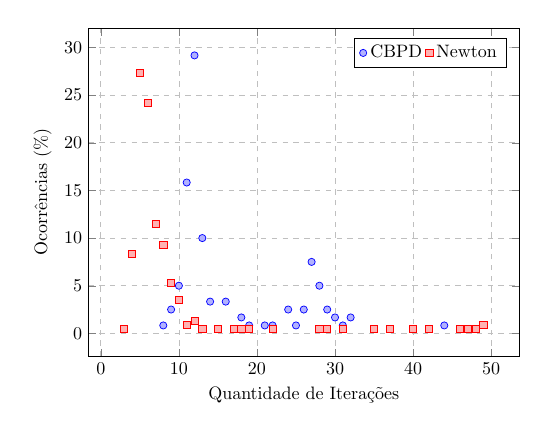
\begin{tikzpicture}[scale = 0.65]
  \begin{axis}[
    width=10cm,
    height=8cm,
    xlabel={Quantidade de Iterações},
    ylabel={Ocorrências (\%)},
    legend style={at={(0.5,-0.2)}, anchor=north, legend columns=-1},
    grid=major,
    grid style=dashed,
    legend pos=north east
  ]

    % First set of data
    \addplot[
      only marks,
      mark=*,
      color=blue,
      fill=blue!30,
    ] coordinates {
      	(13, 10.00)
        (12, 29.17)
        (10, 5.00)
        (11, 15.83)
        (9, 2.50)
        (14, 3.33)
        (16, 3.33)
        (32, 1.67)
        (29, 2.50)
        (27, 7.50)
        (30, 1.67)
        (18, 1.67)
        (31, 0.83)
        (24, 2.50)
        (44, 0.83)
        (28, 5.00)
        (26, 2.50)
        (25, 0.83)
        (21, 0.83)
        (22, 0.83)
        (8, 0.83)
        (19, 0.83)

      };

    % Second set of data
    \addplot[
      only marks,
      mark=square*,
      color=red,
      fill=red!30,
    ] coordinates {
      	(6, 24.23)
        (4, 8.37)
        (5, 27.31)
        (7, 11.45)
        (8, 9.25)
        (9, 5.29)
        (48, 0.44)
        (10, 3.52)
        (22, 0.44)
        (47, 0.44)
        (12, 1.32)
        (31, 0.44)
        (49, 0.88)
        (17, 0.44)
        (11, 0.88)
        (28, 0.44)
        (18, 0.44)
        (40, 0.44)
        (19, 0.44)
        (46, 0.44)
        (29, 0.44)
        (37, 0.44)
        (13, 0.44)
        (42, 0.44)
        (15, 0.44)
        (35, 0.44)
        (3, 0.44)

    };
    \legend{CBPD, Newton}

  \end{axis}
\end{tikzpicture}
\end{center}
